\documentclass[12pt,a4paper]{article}
\usepackage{ucebnice}
\usepackage{hyperref}
\usepackage{url}




\title{Goniometrické rovnice a vzorce}
\author{Ondřej Škubala}
\date{\today}

\begin{document}

\maketitle
\newpage

\section{Úvod}

\subsection*{Goniometrické rovnice a vzorce}

\begin{quotebox}
{$e^{ix} = \cos x + i\sin x$}
{Leonhard Euler — \textit{Introductio in analysin infinitorum} (1748)}
\end{quotebox}


\begin{historicalbox}
\textbf{Historie goniometrických rovnic a vzorců}
Goniometrické rovnice a vzorce mají bohatou historii sahající až do nejstarších civilizací
v nichž se matematika rozvíjela především jako praktický nástroj pro měření, orientaci v prostoru
a popis nebeských jevů.

Zásadní příspěvky k rozvoji goniometrie pocházejí z antického Řecka, kde se matematika
začala chápat jako abstraktní disciplína. Významnou roli zde hrál zejména
\textbf{Hipparchos} z Nikáje (2. století př. n. l.), který je často označován jako "otec trigonometrie".
Ve svých astronomických pracicích sestavil první známé tabulky tětiv kružnice,
které umožňovaly převádět velikosti úhlů na délky tětiv (úseček) a naopak.
Což byly základy pro pozdější vývoj goniometrických funkcí.

Na Hipparchovo dílo navázal \textbf{Ptolemaios} (asi 100–170 n. l.), 
který ve svém monumentálním díle
\href{https://classicalliberalarts.com/resources/PTOLEMY_ALMAGEST_ENGLISH.pdf}{\textit{Almagest}}
shrnuje tehdejší astronomické, matematické poznatky a rozvinul tak trigonometrické poznatky.
Ptolemaios totiž nejen zdokonalil tabulky tětiv, ale také zavedl nové goniometrické vztahy
a vzorce, které se staly základem pro pozdější vývoj goniometrie.

Ve středověku byli antické poznatky dále rozvíjeny zejména v islámském světě.
Matematikové jako \textbf{Al-Battani} (858-929) a \textbf{Al-Khwarizmi} (asi 780-850)
přispěli k rozvoji goniometrických funkcí a tabulek, které byly používány pro astronomické výpočty.

V Indii, kde došlo k zásadnímu konceptuálnímu kroku, k zavedení funkce odpovídajícímu dnešnímu
sinu jako polovině tětivy. Indičtí matematici jako \textbf{Aryabhata} (476-550) a \textbf{Brahmagupta} (598-668)
rozvinuli goniometrické funkce a vztahy, které byly později převzaty a rozšířeny v islámském světě.

Právě z arabských překladů se tyto myšlenky postupně dostaly do Evropy během středověku.
Renesanční období přineslo nový zájem o antickou vědu a matematiku, zejména díky svému propojení 
s astronomií, navigací a kartografií. \textbf{Regiomontanus} (1436-1476) systematicky
zpracovával rovinnou a sférickou goniometrii, čímž položil základy pro moderní trigonometrické metody.
A jeho práce se tak stala standartní pomůckou pro většinu evropských navigátorů a astronomů.

\textbf{Mikuláš Koperník} (1473-1543) ve svém díle \textit{De revolutionibus orbium coelestium}
používal goniometrické rovnice k popisu pohybu planet a formulaci heliocentrického modelu, 
což mělo zásadní dopad na tehdejší vědeckou revoluci.

V 17. století došlo k zásadnímu zlomu v chápání matematických funkcí obecně.
\textbf{Isaac Newton} (1643-1727) a \textbf{Gottfried Wilhelm Leibniz} (1646-1716)
položili základy diferenciálního a integrálního počtu, 
což umožnilo studovat goniometrické funkce z nových perspektiv.
Jako například pomocí Taylorových řad, které umožnily přesnější výpočty a analýzu těchto funkcí.
A to vedlo k hlubšímu pochopení jejich vlastností a aplikací nejen v matematice, ale i v fyzice a inženýrství.

Vrchol tohoto vývoje přišel s prací \textbf{Leona Eulera} (1707-1783),
který goniometrické funkce definitivně zasadil do rámce matematické analýzy.
Euler formulovat slavný vztah (často označován za nejkrásnější rovnici v matematice):
\[e^{ix} = \cos x + i\sin x,\]
který propojuje exponenciální funkci s goniometrickými funkcemi.
Tento vztah nejenže poskytl hluboký vhled do povahy goniometrických funkcí,
ale také otevřel cestu k jejich aplikacím v komplexní analýze, fyzice a inženýrství.
Z tohoto vzorce taktéž vychází známá identita:
\[e^{i\pi} + 1 = 0,\]
která spojuje pět základních matematických konstant ($e$, $i$, $\pi$, $1$, $0$) v jediném elegantním vztahu.

V 19. a 20. století se goniometrické rovnice a vzorce staly nedílnou součástí moderní matematiky
a jejích aplikací v různých vědních oborech, od fyziky přes inženýrství až po počítačovou vědu.
Matematici jako \textbf{Carl Friedrich Gauss} (1777-1855) a \textbf{Joseph Fourier} (1768-1830)
přispěli k dalšímu rozvoji goniometrických funkcí, zejména v oblasti Fourierovy analýzy,
která umožňuje rozklad složitých funkcí na základní goniometrické složky.
Goniometrie se tak postupně stala nástrojem pro měření úhlů v univerzální jazyk, jímž 
lze popisovat široké spektrum jevů v přírodních vědách a technice.

A nakonec ve 20. století a dále, s nástupem počítačů a digitální technologie,
se goniometrické rovnice a vzorce staly klíčovými pro výpočetní metody,
grafiku a simulace. Algoritmy využívající goniometrické funkce jsou
základem pro počítačovou grafiku, zpracování signálů a mnoho dalších aplikací,
které formují náš moderní svět.


\end{historicalbox}    

\section{Základní goniometrické vzorce}

Základní goniometrické vzorce zahrnují vztahy mezi goniometrickými funkcemi,
které jsou užitečné při řešení goniometrických rovnic a při analýze goniometrických funkcí.
Mezi první základní vztahy mezi goniometrickými funkcemi téhož argumentu patří:
\begin{itemize}
    \item $\sin^2 x + \cos^2 x = 1$,
    \item $\tan x \cdot \cot x = 1$.
\end{itemize}

Důkazy těchto vztahů lze odvodit z definic goniometrických funkcí na jednotkové kružnici
nebo pomocí pravoúhlého trojúhelníku.

Pro vztah $\sin^2 x + \cos^2 x = 1$ vyjdeme z faktu jednotkové kružnice.
Mějme jednotkovou kružnici se středem v počátku souřadnicové soustavy.
Nechť úhel $JOK$ má velikost $x$. Bod $K$ na kružnici má souřadnice $K[\cos x, \sin x]$.

\begin{center}
    \begin{tikzpicture}[scale=3, >=latex]
        % ==== DEFINITIONS ====
        \def\angle{150} % Angle in degrees

        % ==== AXES ====
        \draw[<->, thick] (-1.5,0) -- (1.5,0) node[right] {$x$};
        \draw[<->, thick] (0,-1.5) -- (0,1.5) node[above] {$y$};
        
        % ==== UNIT CIRCLE ====
        \draw[thick] (0,0) circle(1);
        
        % ==== ANGLE ====
        \draw[thick] (0,0) -- (\angle:1);
        \draw[thick] (0,0) -- (1,0);
        \draw[thick] (0.2,0) arc(0:\angle:0.2);
        \node at (0.35,0.1) {$x$};
        
        % ==== POINT K ====
        \filldraw[red] (\angle:1) circle(0.02) node[above right] {\footnotesize $K[\cos x, \sin x]$};

        % ==== POINT J ====
        \filldraw[black] (1, 0) circle(0.02) node[below right] {\footnotesize $J[1, 0]$};

        % ==== POINT K_x ====
        \filldraw[black] (cos \angle, 0) circle(0.02) node[below right] {\footnotesize $K_x[\cos x, 0]$};
        
        % ==== DASHED LINE FROM K TO X-AXIS ====
        \draw[dashed] (\angle:1) -- (cos \angle, 0);
    \end{tikzpicture}
\end{center}

Pak v pravoúhlém trojúhelníku $OK_xK$ podle Pythagorovy věty platí:
\[|OK|^2 = |OK_x|^2 + |K_xK|^2.\]

Protože úsečka $OK$ je poloměr jednotkové kružnice, tak $|OK| = 1$, dále platí $|OK_x| = \cos x$ a $|K_xK| = \sin x$.
Dosadíme do Pythagorovy věty:
\[1^2 = (\cos x)^2 + (\sin x)^2,\]
čímž dostaneme požadovaný vztah:
\begin{definitionbox}
    Pro každé $x \in \mathbb{R}$ platí:
    \[\sin^2 x + \cos^2 x = 1.\]
\end{definitionbox}


Pro druhý vztah $\tan x \cdot \cot x = 1$ vyjdeme z definic tangensu a kotangensu:
\[\tan x = \frac{\sin x}{\cos x}, \quad \cot x = \frac{\cos x}{\sin x}.\]
Násobíme tyto dvě rovnice:
\[
\tan x \cdot \cot x
= \frac{\sin x}{\cos x} \cdot \frac{\cos x}{\sin x}
= \frac{\sin x \cdot \cos x}{\cos x \cdot \sin x} = 1.
\]


\begin{definitionbox}
    Pro každé $x \in \mathbb{R}$ platí:
    \[\tan x \cdot \cot x = 1.\]   
\end{definitionbox}



Následně můžeme definovat další vzorce pro dvě čísla $x$ a $y$, které vyjadřují velikost úhlu.

\begin{definitionbox}
    Pro všechna $x$ a $y$ platí \textbf{součtové vzorce:}
    \begin{itemize}
        \item $\sin(x + y) = \sin x \cos y + \cos x \sin y$,
        \item $\sin(x - y) = \sin x \cos y - \cos x \sin y$,
        \item $\cos(x + y) = \cos x \cos y - \sin x \sin y$,
        \item $\cos(x - y) = \cos x \cos y + \sin x \sin y$.
    \end{itemize}
\end{definitionbox}

Dokázat si tyto vzorce můžeme právě pomocí jednotkové kružnice a pravoúhlého trojúhelníku.

Předpokládejme nejprve, že $x, y$ jsou čísla z intervalu $\left\langle 0, \frac{\pi}{2}\right\rangle$ 
a přitom $x > y$. V Kartézské soustavě souřadnic s počátkem $O$ sestrojíme orientovaný úhel
$JOA$ o velikosti $x$ a orientovaný úhel $JOB$ o velikosti $y$. 


% DVA OBRÁZKY (tikz) vedle sebe
\begin{center}
    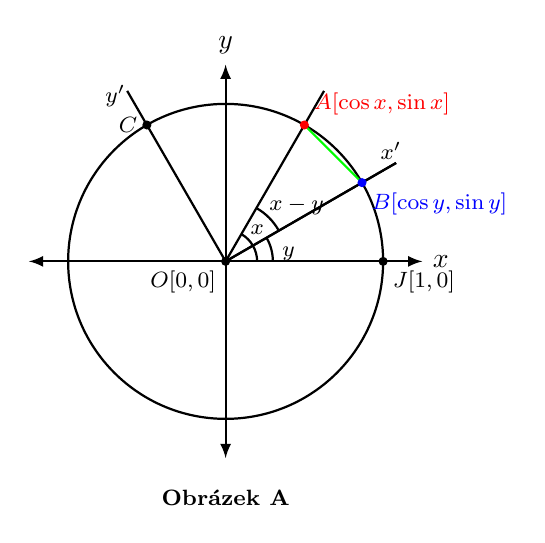
\begin{tikzpicture}[scale=1, >=latex]
        % Až to budeš opravovat, tak buď rád, 
        % za to, že sis to tak hezky popsal, 
        % protože jinak by ses z toho jinak posral. :D 


        % ==== DEFINITIONS ====
        \def\angleX{60} % Angle x in degrees
        \def\angleY{30} % Angle y in degrees

        % ==== UNIT CIRCLE ====
        \draw[thick] (0,0) circle(2);

        % ==== AXES ====
        \draw[<->, thick] (-2.5,0) -- (2.5,0) node[right] {$x$};
        \draw[<->, thick] (0,-2.5) -- (0,2.5) node[above] {$y$};

        % ==== ANGLE x ====
        \draw[thick] (0,0) -- (\angleX:2.5);
        
        % ==== ANGLE Y ====
        \draw[thick] (0,0) -- (\angleY:2.5);

        % ==== ANGLE X - Y ====
        \draw[thick] (0,0) -- ({\angleX - \angleY}:2.5);

        % ==== GREEN LINE FROM A to B ====
        \draw[thick, green] (\angleX:2) -- (\angleY:2);

        % ==== POINTS A and B ====
        \filldraw[red] (\angleX:2) circle(0.05) node[above right] {\footnotesize $A[\cos x, \sin x]$};
        \filldraw[blue] (\angleY:2) circle(0.05) node[below right] {\footnotesize $B[\cos y, \sin y]$};

        % ==== POINT J and O ====
        \filldraw[black] (2, 0) circle(0.05) node[below right] {\footnotesize $J[1, 0]$};
        \filldraw[black] (0, 0) circle(0.05) node[below left] {\footnotesize $O[0, 0]$};

        % ==== ANGLE MARKS ====
        \draw[thick] (0.4,0) arc(0:\angleX:0.4);
        \node at (0.4,0.4) {\footnotesize $x$};
        \draw[thick] (0.6,0) arc(0:\angleY:0.6);
        \node at (0.8,0.1) {\footnotesize $y$};
        \draw[thick] (0.67,0.4) arc(\angleY:\angleX:0.75);
        \node at (0.9,0.7) {\footnotesize $x - y$};

        % ==== MARK x' ====
        \node at (2.1, 1.4) {\footnotesize $x'$};

        % ==== POINT C ====
        \filldraw[black] ({\angleY + 90}:2) circle(0.05) node[left] {\footnotesize $C$};

        % ==== LINE FROM O to C ====
        \draw[thick] (0,0) -- ({\angleY + 90}:2.5);

        % ==== MARK y' ====
        \node at (-1.4, 2.1) {\footnotesize $y'$};

        % ==== TITLE ====
        \node at (0, -3) {\footnotesize \textbf{Obrázek A}};
    \end{tikzpicture}
    \hspace{2cm}
    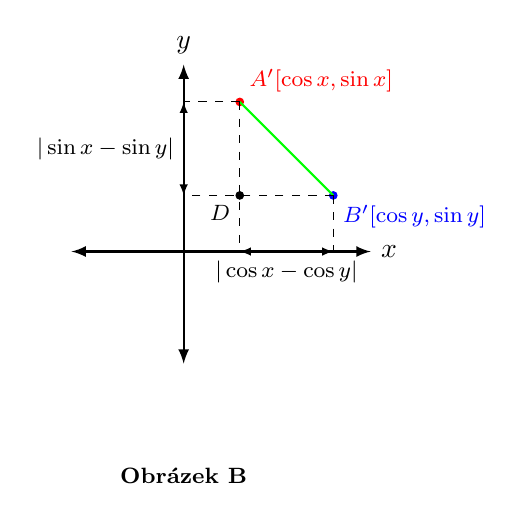
\begin{tikzpicture}[scale=0.95, >=latex]
        % ==== DEFINITIONS ====
        \def\Ax{0.75} % Ax length
        \def\Ay{2} % Ay length
        \def\Bx{2} % Bx length
        \def\By{0.75} % By length

        % ==== AXIS ====
        \draw[<->, thick] (-1.5,0) -- (2.5,0) node[right] {$x$};
        \draw[<->, thick] (0,-1.5) -- (0,2.5) node[above] {$y$};

        % ==== POINTS A and B ====
        \filldraw[red] (\Ax, \Ay) circle(0.05) node[above right] {\footnotesize $A'[\cos x, \sin x]$};
        \filldraw[blue] (\Bx, \By) circle(0.05) node[below right] {\footnotesize $B'[\cos y, \sin y]$};

        % ==== GREEN LINE FROM A to B ====
        \draw[thick, green] (\Ax, \Ay) -- (\Bx, \By);
        % ==== DASHED LINES FROM A and B TO AXES ====
        \draw[dashed] (\Bx, \By) -- (\Bx, 0);
        \draw[dashed] (\Ax, \Ay) -- (0, \Ay);
        \draw[dashed] (\Bx, \By) -- (0, \By);
        \draw[dashed] (\Ax, \Ay) -- (\Ax, 0); 

        % ==== POINT D ====
        \filldraw[black] (\By, \Ax) circle(0.05) node[below left] {\footnotesize $D$};

        % ==== LENGTH OF ordinate ====
        \draw[<->] (\Ax, 0) -- (\Bx, 0) node[midway, below] {\footnotesize $|\cos x - \cos y|$};
        \draw[<->] (0, \Ay) -- (0, \By) node[midway, left] {\footnotesize $|\sin x - \sin y|$};

        % ==== TITLE ====
        \node at (0, -3) {\footnotesize \textbf{Obrázek B}};

    \end{tikzpicture}

\end{center}

Bod J má souřadnice $J[1, 0]$, bod A má souřadnice $A[\cos x, \sin x]$, bod $B$ má souřadnice $B[\cos y, \sin y]$.
Body $A, B$ vedeme rovnoběžky s osami souřadnic. V pravoúhlém trojúhelníku $OAB$ 
pak podle podobnosti trojúhelníků $ABD$ (Obrázek B):
\[
|AB|^2 = |AD|^2 + |BD|^2,
\]
po dosazení délek přepon:
\[
|AB|^2 = |\cos y - \cos x|^2 + |\sin x - \sin y|^2
\]
a to lze upravit postupně na:
\[
|AB|^2 = 2\left(1 - \cos x \cos y - \sin x \sin y\right)
\]

\begin{center}
    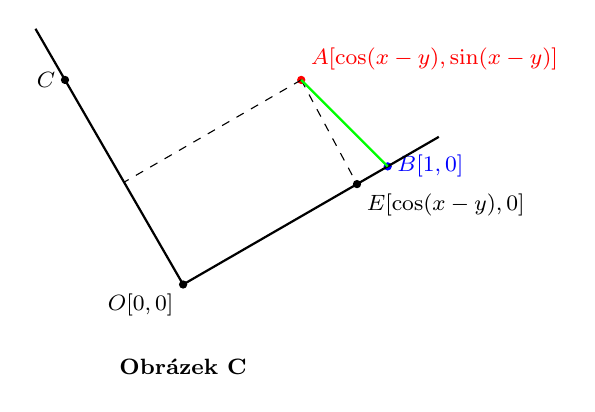
\begin{tikzpicture}[scale=1.5, >=latex]
        % ==== DEFINITIONS ====
        \def\angleX{60} % Angle x in degrees
        \def\angleY{30} % Angle y in degrees

        
        % ==== POINT O ====
        \filldraw[black] (0, 0) circle(0.03) node[below left] {\footnotesize $O[0, 0]$};

        % ==== POINT C ====
        \filldraw[black] ({\angleY + 90}:2) circle(0.03) node[left] {\footnotesize $C$};

        % ==== POINT A and B ====
        \filldraw[red] ({\angleX}:2) circle(0.03) node[above right] {\footnotesize $A[\cos (x - y), \sin (x - y)]$};
        \filldraw[blue] ({\angleY}:2) circle(0.03) node[right] {\footnotesize $B[1,0]$};

        % ==== LINE FROM O to C ====
        \draw[thick] (0,0) -- ({\angleY + 90}:2.5);
        % ==== LINE FROM O to B ====
        \draw[thick] (0,0) -- ({\angleY}:2.5);

        % ==== PERPENDICULAR LINE FROM A TO OC ====
        \draw[dashed] ({\angleX}:2) -- ({\angleY + 90}:1);
        % ==== PERPENDICULAR LINE FROM A TO OB ====
        \draw[dashed] ({\angleX}:2) -- ({\angleY}:1.7);

        % ==== GREEN LINE FROM A to B ====
        \draw[thick, green] ({\angleX}:2) -- ({\angleY}:2);

        % ==== POINT E on OB====
        \filldraw[black] ({\angleY}:1.7) circle(0.03) node[below right]  {\footnotesize $E[\cos(x-y), 0]$};
    
        % ==== TITLE ====
        \node at (0, -0.7) {\footnotesize \textbf{Obrázek C}};
    \end{tikzpicture}
\end{center}


Otočíme-li soustavu souřadnic Oxy o úhel $JOB$ (velikosti $y$) proti směru hodinových ručiček, 
přejde osa $x$ na osu $x' = OB$ a osa $y$ na osu $y' = OC$, přičemž $x' \perp y'$.
Pro body $A, B$ v této nové soustavě bude platit: $B[1,0]$, $A[\cos(x - y), \sin(x - y)]$.
Bodem $A$ vedeme rovnoběžky s osami $x', y'$.
V pravoúhlém trojúhelníku $AEB$ (Obrázek C) platí:
\[
|BE| = |1 - \cos (x-y)|,
\]
\[
|AE| = |\sin (x-y)|.
\]

Podle Pythagorovy věty tedy platí:
\[
\begin{aligned}
|AB|^2 &= |BE|^2 + |AE|^2 , \\ [0.5em]
|AB|^2 &= |1 - \cos (x-y)|^2 + |\sin (x-y)|^2.    
\end{aligned}
\]

Tedy máme dvě rovnice pro $|AB|^2$:
\[
\begin{aligned}
|AB|^2 &= 2\left(1 - \cos x \cos y - \sin x \sin y\right), \\[0.5em]
|AB|^2 &= |1 - \cos (x-y)|^2 + |\sin (x-y)|^2.
\end{aligned}
\]

Po porovnáním těchto dvou rovnic a úpravě dostaneme:
\[
\cos (x-y) = \cos x \cos y + \sin x \sin y,
\]
Tímto jsme si dokázali čtvrtý součtový vzorec. Ostatní tři vzorce lze dokázat obdobně.
My si však ještě ukážeme jak lze odvodit první součtový vzorec ze čtvrtého.

\medskip
Důkaz prvního součtového vzorce z faktu: $\sin x = \cos \left(\frac{\pi}{2} - x \right)$:
\[
\begin{aligned}
    \sin (x + y)    &= \cos \left[\frac{\pi}{2} - (x + y) \right] = \\[0.5em]
                    &= \cos \left[\frac{\pi}{2} - x - y \right] = \\[0.5em]
                    &= \cos \left[\left(\frac{\pi}{2} - x\right) - y \right] = \\[0.5em]
                    &= \cos \left(\frac{\pi}{2} - x\right) \cos y + \sin \left(\frac{\pi}{2} - x\right) \sin y = \\[0.5em]
                    &= \sin x \cos y + \cos x \sin y.
\end{aligned}
\]
A tím jsme dokázali i první vzorec ze součtových vzorců. Dokázání zbylých součtových vzorců nechám na BONUSOVÝ příklad na procvičování. 

%
% ZDE JE TEN PŘÍKLAD
% ZDE JE TEN PŘÍKLAD
%

\begin{notebox}
    Tyto vzorce je nutné si zapamatovat, protože jsou často využívány při řešení goniometrických rovnic,
    při analýze goniometrických funkcí a u komplexních čísel.
\end{notebox}

Následně můžeme obdobně definovat i další vzorce pro součet a rozdíl hodnot goniometrických funkcí.

\begin{definitionbox}
    Pro všehna $x$ a $y$ platí \textbf{součty a rozdíly hodnot goniometrických funkcí:}
    \begin{itemize}
        \item $\sin x + \sin y = 2 \cdot \sin \frac{x+y}{2} \cdot \cos \frac{x-y}{2}$,
        \item $\sin x - \sin y = 2 \cdot \cos \frac{x+y}{2} \cdot \sin \frac{x-y}{2}$,
        \item $\cos x + \cos y = 2 \cdot \cos \frac{x+y}{2} \cdot \cos \frac{x-y}{2}$,
        \item $\cos x - \cos y = -2 \cdot \sin \frac{x+y}{2} \cdot \sin \frac{x-y}{2}$.
    \end{itemize}

\end{definitionbox}

Tyto vzorce jsou užitečné při řešení goniometrických rovnic a při analýze goniometrických funkcí. 
Avšak jejich důkazy jsou poněkud složitější a vyžadují hlubší znalosti goniometrie a algebraických manipulací.

A poslední vzorce, které zde uvedeme, jsou pro dvojnásobný a poloviční úhel.
\begin{definitionbox}
    Pro všechna $x$ platí \textbf{vzorce pro dvojnásobný a poloviční úhel:}
    \begin{itemize}
        \item $\sin 2x = 2 \sin x \cos x$,
        \item $\cos 2x = \cos^2 x - \sin^2 x = 2\cos^2 x - 1 = 1 - 2\sin^2 x$,
        \item $\left|\sin \frac{x}{2}\right| = \left|\sqrt{\frac{1 - \cos x}{2}}\right|$,
        \item $\left|\cos \frac{x}{2}\right| = \left|\sqrt{\frac{1 + \cos x}{2}}\right|$.
    \end{itemize}
\end{definitionbox}

Tyto vzorce využijeme například při zjednodušování goniometrických výrazů
nebo při řešení goniometrických rovnic.

\begin{examplebox}
    \textbf{Zjednodušte výraz}
    \[
    \left(1 + \cos x\right)\left(1 - \cos x\right)
    \]
    a určete jeho definiční obor.
    
    \medskip
    \textbf{Řešení:}
    Využijeme vzorce $a^2 - b^2 = (a+b)(a-b)$:
    \[
    \left(1 + \cos x\right)\left(1 - \cos x\right) = 1^2 - (\cos x)^2 = 1 - \cos^2 x.
    \]
    Dále využijeme základní goniometrický vztah $\sin^2 x + \cos^2 x = 1$:
    \[
    1 - \cos^2 x = \sin^2 x.
    \]
    Tedy zjednodušený výraz je $\sin^2 x$.

    \medskip
    Definiční obor výrazu je $D(f)=\mathbb{R}$, protože goniometrické funkce jsou definovány pro všechna reálná čísla $x$.
\end{examplebox}

\begin{examplebox}
    \textbf{Zjednodušte výraz:}
    \[
    \sin^4 x + 2\sin^2 x \cos^2 x + \cos^4 x
    \]
    a určete jeho definiční obor.

    \medskip
    \textbf{Řešení:}
    Využijeme vzorec pro čtverec součtu $(a+b)^2 = a^2 + 2ab + b^2$:
    \[
    \sin^4 x + 2\sin^2 x \cos^2 x + \cos^4 x = (\sin^2 x + \cos^2 x)^2.
    \]
    Dále využijeme základní goniometrický vztah $\sin^2 x + \cos^2 x = 1$:
    \[
    (\sin^2 x + \cos^2 x)^2 = 1^2 = 1.
    \]
    Tedy zjednodušený výraz je $1$.

    \medskip
    Definiční obor výrazu je $D(f)=\mathbb{R}$, protože goniometrické funkce jsou definovány pro všechna reálná čísla $x$.
\end{examplebox}

\begin{examplebox}
    \textbf{Zjednodušte výraz:}
    \[
    \frac{1}{1 + \cot x} - \frac{\tan x}{1 + \tan x}
    \]
    a určete jeho definiční obor.

    \medskip
    \textbf{Řešení:}
    Nejprve využijeme faktu, že $\cot x = \dfrac{1}{\tan x}$:
    \[
    \frac{1}{1 + \cot x} - \frac{\tan x}{1 + \tan x} = \frac{1}{1 + \frac{1}{\tan x}} - \frac{\tan x}{1 + \tan x}.
    \]
    Následně upravíme první zlomek:
    \[
    \frac{1}{1 + \frac{1}{\tan x}} = \frac{\tan x}{\tan x + 1}.
    \]
    Tedy máme:
    \[
    \frac{\tan x}{\tan x + 1} - \frac{\tan x}{1 + \tan x} = \frac{\tan x - \tan x}{1 + \tan x} = 0.
    \]
    Tedy zjednodušený výraz je $0$.
    
    \medskip
    Definiční obor výrazu je $D(f)=\mathbb{R} \setminus \left\{k\pi + \dfrac{\pi}{2}, k \in \mathbb{Z}\right\}$,
    protože tangens a kotangens nejsou definovány pro tyto hodnoty $x$.
\end{examplebox}

\begin{examplebox}
    Určete hodnoty všech goniometrických funkcí v bodě $x$, jestliže platí $\cot x = \sqrt{2}$
    a zároveň $x \in \left(0, \frac{\pi}{2}\right)$.

    \medskip
    \textbf{Řešení:}
    Z identity $\cot x = \frac{1}{\tan x}$:
    \[
    \tan x = \frac{1}{\cot x} = \frac{1}{\sqrt{2}} = \frac{\sqrt{2}}{2}.
    \]

    Následně využijeme vztah $\tan x = \frac{\sin x}{\cos x}$:
    \[
    \frac{\sin x}{\cos x} = \frac{\sqrt{2}}{2} \implies \sin x = \frac{\sqrt{2}}{2} \cos x.
    \]
    Dále využijeme základní goniometrický vztah $\sin^2 x + \cos^2 x = 1$:
    \[
    \begin{aligned}
        \sin^2 x + \cos^2 x &= 1 && \big/ : \sin^2 x \\[0.5em]
        \frac{\sin^2 x}{\sin^2 x} + \frac{\cos^2 x}{\sin^2 x} &= \frac{1}{\sin^2 x} \\[0.5em]
        \cot^2 x + 1 &= \frac{1}{\sin^2 x}
    \end{aligned}
    \]
    Vyjádříme $\sin^2 x$ a dosadíme hodnotu $\cot x = \sqrt{2}$:
    \[
    \sin^2 x = \frac{1}{\cot^2 x + 1} = \frac{1}{(\sqrt{2})^2 + 1} = \frac{1}{2 + 1} = \frac{1}{3}.
    \]
    A jako poslední odmocníme a vyjde nám tedy:
    \[
    |\sin x| = \frac{1}{\sqrt{3}}.
    \]

    V intervalu $\left(0, \frac{\pi}{2}\right)$ je $\sin x$ kladné, takže:
    \[
    \sin x = \frac{1}{\sqrt{3}} = \frac{\sqrt{3}}{3}.
    \]
    Následně dosadíme zpět do rovnice $\sin x = \frac{\sqrt{2}}{2} \cos x$ a vyjádříme $\cos x$:
    \[
    \frac{1}{\sqrt{3}} = \frac{\sqrt{2}}{2} \cos x \implies \cos x = \frac{2}{\sqrt{6}} = \frac{\sqrt{6}}{3}.
    \]
    
    \medskip
    Tím jsme dopočítali všechny goniometrické funkce v bodě $x$:
    \begin{itemize}
        \item $\sin x = \frac{1}{\sqrt{3}}$,
        \item $\cos x = \frac{2}{\sqrt{6}}$,
        \item $\tan x = \frac{\sqrt{2}}{2}$,
        \item $\cot x = \sqrt{2}$,
    \end{itemize}
\end{examplebox}

Tím máme za sebou základní goniometrické vzorce a jejich využití při zjednodušování výrazů
a výpočtu hodnot goniometrických funkcí. V další kapitole se podíváme na goniometrické rovnice
a jejich řešení.

\section{Goniometrické rovnice}

\important{Goniometrické rovnice} jsou rovnice, které obsahují goniometrické funkce jako
\textbf{sinus}, \textbf{kosinus}, \textbf{tangens} nebo \textbf{kotangens}.

Základní goniometrické rovnice je zapsaná ve tvaru $f(x) = a$, kde $f(x)$ je goniometrická funkce
a $a$ je reálné číslo. Cílem je najít všechna řešení $x$, která splňují tuto rovnici.

Základní řešení goniometrických rovnic je množina všech hodnot $x$, které splňují rovnici v jednom cyklu goniometrické funkce.
Tedy například pro sinus a kosinus je základní řešení v intervalu $\langle 0, 2\pi)$.

\begin{examplebox}
    Řešte goniometrickou rovnici:
    \[
    \sin x = \frac{\sqrt{3}}{2}.
    \]

    \medskip
    \textbf{Řešení:}
    Nejprve najdeme základní řešení v intervalu $\langle 0, 2\pi)$.
    Hodnota $\sin x = \frac{\sqrt{3}}{2}$ nastává pro $x = \frac{\pi}{3}$ a $x = \frac{2\pi}{3}$.
    Tedy základní řešení je:
    \[
    x_1 = \frac{\pi}{3}, \quad x_2 = \frac{2\pi}{3}.
    \]
    Následně určíme obecné řešení goniometrické rovnice.
    Pro sinus platí, že obecné řešení je dáno vzorcem:
    \[
    K = \bigcup_{k \in \mathbb{Z}}  \left\{ \frac{\pi}{3} + k \cdot 2\pi, \frac{2\pi}{3} + k \cdot 2\pi\right\},
    \]

    Nejlépe je ověřit si řešení na jednotkové kružnici:
    \begin{center}
        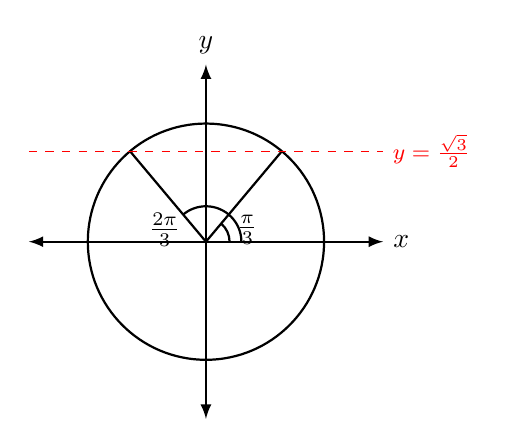
\begin{tikzpicture}[scale=1.5, >=latex]
            % ==== DEFINITIONS ====
            \def\angleOne{50} % Angle in degrees
            \def\angleTwo{130} % Angle in degrees

            % ==== AXES ====
            \draw[<->, thick] (-1.5,0) -- (1.5,0) node[right] {$x$};
            \draw[<->, thick] (0,-1.5) -- (0,1.5) node[above] {$y$};
            
            % ==== UNIT CIRCLE ====
            \draw[thick] (0,0) circle(1);
            
            % ==== ANGLE ONE ====
            \draw[thick] (0,0) -- (\angleOne:1);
            \draw[thick] (0,0) -- (1,0);
            \draw[thick] (0.2,0) arc(0:\angleOne:0.2);
            \node at (0.35,0.1) {$\frac{\pi}{3}$};
            
            % ==== ANGLE TWO ====
            \draw[thick] (0,0) -- (\angleTwo:1);
            \draw[thick] (0.3,0) arc(0:\angleTwo:0.3);
            \node at (-0.35,0.1) {$\frac{2\pi}{3}$};

            % ==== LINE y=sqrt(3)/2 ====
            \draw[dashed, red] (-1.5, {sin(\angleOne)}) -- (1.5, {sin(\angleTwo)}) node[right] {\footnotesize $y=\frac{\sqrt{3}}{2}$};

        \end{tikzpicture}
    \end{center}
\end{examplebox}    

Jak jste si všimnout, tak zápis množiny řešení goniometrických rovnic je poněkud odlišný
od běžných rovnic. To je způsobeno tím, že goniometrické funkce jsou periodické,
což znamená, že se jejich hodnoty opakují v pravidelných intervalech.
Tedy pro každé základní řešení existuje nekonečně mnoho dalších řešení,
která lze získat přičtením celých násobků periody goniometrické funkce.

Ten symbol
\[
    \bigcup_{k \in \mathbb{Z}} = \{\text{úhly}\}
\] 
označuje sjednocení množin všech řešení
pro všechna celá čísla $k$. Tímto způsobem můžeme vyjádřit nekonečnou množinu řešení goniometrické rovnice.

\subsubsection*{Řešení pomocí substituce}
Rovnice mohou být složitější a mohou obsahovat více goniometrických funkcí
nebo kombinace goniometrických funkcí s jinými matematickými operacemi.
Takové goniometrické rovnice mohou vyžadovat kombinaci různých technik,
jako je použití \textbf{goniometrických vzorců}, \textbf{substituce} nebo \textbf{algebraických manipulací}.


\begin{examplebox}
    Řešte rovnici:
    \[
    2 \sin (3x + \pi) = -1
    \].

    \medskip
    \textbf{Řešení:}
    Rovnici budeme řešit substitucí za proměnnou $y = 3x + \pi$:
    \[
    \begin{aligned}
        2 \sin y &= -1 && \big/ : 2 \\[0.5em]
        \sin y &= -\frac{1}{2}
    \end{aligned}
    \]

    Tuto rovnici již umíme řešit. Nejprve najdeme základní řešení v intervalu $\langle 0, 2\pi)$.
    Hodnota $\sin y = -\frac{1}{2}$ nastává pro $y = \frac{7\pi}{6}$ a $y = \frac{11\pi}{6}$.
    Tedy základní řešení je:
    \[
    y_1 = \frac{7\pi}{6}, \quad y_2 = \frac{11\pi}{6}.
    \]
    Nyní musíme udělat návrat k původní proměnné $x$:
    \[
    \begin{aligned}
        3x_1 + \pi &= \frac{7\pi}{6} + 2k\pi \\[0.5em]
        3x_2 + \pi &= \frac{11\pi}{6} + 2k\pi
    \end{aligned}
    \]
    Z těchto rovnic pak vyjádříme obecné řešení pro $x$:
    \[
    \begin{aligned}
        3x_1 &= \frac{7\pi}{6} - \pi + 2k\pi = \frac{7}{18}\pi + \frac{1}{3}\left(2k - 1\right)\pi, \\[0.5em]
        3x_2 &= \frac{11\pi}{6} - \pi + 2k\pi = \frac{11}{18}\pi + \frac{1}{3}\left(2k - 1\right)\pi.
    \end{aligned}
    \]
    Což ještě můžeme upravit jako:
    \[
    \begin{aligned}
        x_1 &= \frac{\pi}{18} + \frac{2}{3}k\pi, \\[0.5em]
        x_2 &= \frac{5\pi}{18} + \frac{2}{3}k\pi.
    \end{aligned}
    \]
    A tedy obecné řešení je:
    \[
    K = \bigcup_{k \in \mathbb{Z}} \left\{ \frac{\pi}{18} + \frac{2}{3}k\pi, \frac{5\pi}{18} + \frac{2}{3}k\pi \right\}.
    \]
\end{examplebox}

Tímto jsme si ukázali základní principy řešení goniometrických rovnic.
V dalších kapitolách se budeme věnovat specifickým typům goniometrických rovnic
a jejich řešení, včetně rovnic s více goniometrickými funkcemi,
kombinací goniometrických funkcí a aplikací goniometrických rovnic v různých oblastech matematiky a vědy.

\begin{examplebox}
    Řešte rovnici:
    \[
    \sin 2x = \cos 3x \cdot \sin 2x.
    \]

    \medskip
    \textbf{Řešení:}

    Nejprve upravíme rovnici:
    \[
    \begin{aligned}
        \sin 2x &= \cos 3x \cdot \sin 2x  && \big/ : -\cos 3x \cdot \sin 2x \\[0.5em]
        \sin 2x - \cos 3x \cdot \sin 2x &= 0 \\[0.5em]
        \sin 2x (1 - \cos 3x) &= 0
    \end{aligned}
    \]
    Nyní máme součin dvou členů roven nule, což znamená, že alespoň jeden z těchto členů musí být roven nule.
    Tedy řešíme dvě rovnice:
    \[
    \sin 2x = 0, \quad \text{nebo} \quad 1 - \cos 3x = 0.
    \]
    Začneme první rovnicí:
    \[
    \sin 2x = 0.
    \]
    Opět použijeme substituci $u = 2x$:
    \[
    \sin u = 0.
    \]
    Známe základní řešení $\sin u = 0$ v intervalu $\langle 0, 2\pi)$, což je $u = 0$ a $u = \pi$.
    Obecné řešení po návratu substituce je tedy:
    \[
    2x = k\pi \implies x = \frac{k\pi}{2}, \quad k \in \mathbb{Z}.
    \]

    \medskip
    Nyní řešíme druhou rovnici:
    \[
    1 - \cos 3x = 0 \implies \cos 3x = 1.
    \]
    Znovu použijeme substituci $v = 3x$:
    \[
    \cos v = 1.
    \]
    Známe základní řešení $\cos v = 1$ v intervalu $\langle 0, 2\pi)$, což je $v = 0$.
    Obecné řešení po návratu substituce je tedy:
    \[
    3x = 2l\pi \implies x = \frac{2l\pi}{3}, \quad l \in \mathbb{Z}.
    \]
    
    \medskip
    Máme tedy tyto dvě řešení:
    \[
    x_1 = \frac{k\pi}{2}, \quad k \in \mathbb{Z},
    \quad
    x_2 = \frac{2l\pi}{3}, \quad l \in \mathbb{Z}.
    \]
    Vzhledem k tomu, že $k$ a $l$ jsou nezávislé proměnné, můžeme je sjednotit do jedné množiny řešení:
    \[
    \bigcup_{k \in \mathbb{Z}} \left\{k \cdot \frac{\pi}{2}\right\} \cup \bigcup_{l \in \mathbb{Z}} \left\{l \cdot \frac{2\pi}{3}\right\}.
    \]

    Což lze zapsat jako jednu množinu řešení:
    \[
    K = \bigcup_{m \in \mathbb{Z}} \left\{\frac{1}{2}\pi m, \frac{2}{3} \pi m \right\}.
    \]
\end{examplebox}    

\begin{notebox}
    \textbf{Poznámka:}

    Při řešení goniometrických rovnic je důležité si uvědomit, že dělení goniometrickou funkcí může vést ke ztrátě řešení.
    A to z důvodu, že goniometrické funkce mohou nabývat hodnoty nula.
    Proto je vždy lepší upravit rovnici tak, aby se goniometrická funkce nevyskytovala ve jmenovateli.
\end{notebox}


Nyní máme za sebou základní principy řešení goniometrických rovnic.
A ukážeme si jeden příklad na závěr této kapitoly, 
který vyžaduje důkladnější a pečlivou práci a systematický postup.

\begin{examplebox}
    Řešte rovnici:
    \[
    \cos 2x - \sin 2x = \left(\sin x + \cos x\right)^2.
    \]
    \medskip
    \textbf{Řešení:}

    Nejprve upravíme levou stranu rovnice pomocí vzorců a pravou stranu umocníme:
    \[
    \begin{aligned}
        \cos^2 x - \sin^2 x - 2\sin x \cos x &= \sin^2 x + 2\sin x \cos x + \cos^2 x \\[0.5em]
        0 &= 2\sin^2 x + 4\sin x \cos x  && \big/ : 2 \\[0.5em]
        0 &= \sin^2 x + 2\sin x \cos x \\[0.5em]
        0 &= \sin x (\sin x + 2\cos x)
    \end{aligned}
    \]

    Dostali jsme součin dvou členů roven nule, což znamená, že alespoň jeden z těchto členů musí být roven nule.
    Tedy řešíme dvě rovnice:
    \[
    \sin x = 0  \quad \vee  \quad \sin x + 2\cos x = 0.
    \]

    Začneme první rovnicí:
    \[
    \sin x = 0.
    \]
    Známe základní řešení $\sin x = 0$ v intervalu $\langle 0, 2\pi)$, což je $x = 0$ a $x = \pi$.
    Obecné řešení je tedy:
    \[
    x_1 = k \cdot 180^\circ, \quad k \in \mathbb{Z}.
    \]

    \medskip
    Nyní řešíme druhou rovnici:
    \[
    \sin x + 2\cos x = 0.
    \]
    Vyjádříme $\sin x$:
    \[
    \sin x = -2\cos x.
    \]
    Následně vydělíme obě strany rovnice $\cos x$ (a musíme určit podmínku, že $\cos x \neq 0$):
    \[
    \frac{\sin x}{\cos x} = -2.
    \]
    Tedy máme:
    \[
    \tan x = -2.
    \]
    Nyní najdeme základní řešení $\tan x = -2$ v intervalu $\langle 0, 2\pi)$.
    Hodnota $\tan x = -2$ nastává pro $x = \arctan(-2) + k\pi$.
    Tedy základní řešení je:
    \[
    x_2 = \arctan(-2) + k\pi, \quad k \in \mathbb{Z}.
    \]
    Hodnota $\arctan(-2)$ odpovídá úhlu v druhém $116^\circ 34'$ a čtvrtém kvadrantu $-63^\circ 26'$.
    \medskip
    Což tedy můžeme zapsat jako:
    \[
    x_2 = 116^\circ 34' + k\cdot 180^\circ, \quad k \in \mathbb{Z}, \\
    \]
    \[
    x_3 = -63^\circ 26' + k\cdot 180^\circ, \quad k \in \mathbb{Z}.
    \]

    \medskip
    Máme tedy tyto tři řešení:
    \[
    x_1 = k \cdot 180^\circ, \quad k \in \mathbb{Z},
    \]
    \[
    x_2 = 116^\circ 34' + k\cdot 180^\circ, \quad k \in \mathbb{Z},
    \]
    \[
    x_3 = -63^\circ 26' + k\cdot 180^\circ, \quad k \in \mathbb{Z}.
    \]


    \bigskip
    Protože jsme dělili rovnici $\cos x$ a tato úprava není ekvivalentní,
    musíme zkontrolovat, zda některé z nalezených řešení nevedou k dělení nulou.
    A protože perioda funkcí $\sin x$ a $\cos x$ je $360^\circ$, musíme zkoušky provádět pro:
    \[
    x_1 = k \cdot 360^\circ,
    \]
    \[
    x_2 = 116^\circ 34' + k\cdot 360^\circ,
    \]
    \[
    x_3 = -63^\circ 26' + k\cdot 360^\circ \rightarrow 296^\circ 34' + k\cdot 360^\circ,
    \]
    \[
    x_4 = 180^\circ + k\cdot 360^\circ.
    \]

    \textbf{Zkouška:}
    \[
    L(x_1) = \cos 0 - \sin 0 = 1 - 0 = 1,
    \]
    \[
    P(x_1) = (\sin 0 + \cos 0)^2 = (0 + 1)^2 = 1,
    \]
    \[
    L(x_1) = P(x_1) \quad \checkmark
    \]

    \medskip
    \[
    L(x_2) = \cos 233^\circ 8' - \sin 233^\circ 8' = -0.6018 + 0.7986 = 0.1968,
    \]
    \[
    P(x_2) = (\sin 116^\circ 34' + \cos 116^\circ 34')^2 = (0.8988 - 0.4384)^2 = 0.1968,
    \]
    \[
    L(x_2) = P(x_2) \quad \checkmark
    \]

    \medskip
    \[
    L(x_3) = \cos 593^\circ 8' - \sin 593^\circ 8' = 0.6018 + 0.7986 = 1.4004,
    \]
    \[
    P(x_3) = (\sin 296^\circ 34' + \cos 296^\circ 34')^2 = (-0.8988 - 0.4384)^2 = 1.4004,
    \]
    \[
    L(x_3) = P(x_3) \quad \checkmark
    \]

    \medskip
    \[
    L(x_4) = \cos 2 \left(180^\circ\right) - \sin 2 \left(180^\circ\right) = \cos 360^\circ - \sin 360^\circ = 1 - 0 = 1
    \]
    \[
    P(x_4) = (\sin 180^\circ + \cos 180^\circ)^2 = (0 - 1)^2 = 1,
    \]
    \[
    L(x_4) = P(x_4) \quad \checkmark
    \]

    Všechny nalezená řešení tedy vyhovují původní rovnici.
    A tedy konečná množina řešení je:
    \[
    K = \bigcup_{k \in \mathbb{Z}} \left\{k \cdot 180^\circ, 116^\circ 34' + k\cdot 180^\circ, -63^\circ 26' + k\cdot 180^\circ\right\}.
    \]



\end{examplebox}



\section{Goniometrické nerovnice}
Goniometrické nerovnice jsou nerovnice, které obsahují goniometrické funkce jako
\textbf{sinus}, \textbf{kosinus}, \textbf{tangens} nebo \textbf{kotangens} a mají tvar:

\begin{definitionbox}
    \textbf{Goniometrické nerovnice} jsou nerovnice ve tvaru:
    \[
    f(x) > a, \quad f(x) < a, \quad f(x) \geq a, \quad f(x) \leq a,
    \]
    kde $f(x)$ je goniometrická funkce a $a$ je reálné číslo.
\end{definitionbox}

Řešení goniometrických nerovnic zahrnuje několik kroků:
\begin{enumerate}[label=\arabic*.]
    \item \textbf{Úprava nerovnice:} Podobně jako u goniometrických rovnic je často užitečné upravit nerovnici pomocí goniometrických vzorců.
    \item \textbf{Najít kritické body:} Určete hodnoty $x$, kde goniometrická funkce dosahuje hodnoty $a$.
    \item \textbf{Intervaly řešení:} Rozdělte číselnou osu na intervaly pomocí kritických bodů a určete, ve kterých intervalech nerovnice platí.
    \item \textbf{Zápis řešení:} Vyjádřete množinu řešení pomocí intervalů nebo sjednocení množin.
    \item \textbf{Kontrola řešení:} Ověřte nalezená řešení dosazením zpět do původní nerovnice.
\end{enumerate}


\begin{examplebox}
    Mějme goniometrickou nerovnici:
    \[
    \sin x \le -0.5.
    \]
    \medskip
    \textbf{Řešení:}
    Před tím, nežto budeme řešit si to ukážeme na jednotkové kružnici, kde je vidět, kdy je hodnota sinu menší nebo rovna $-0.5$.

    \begin{center}
        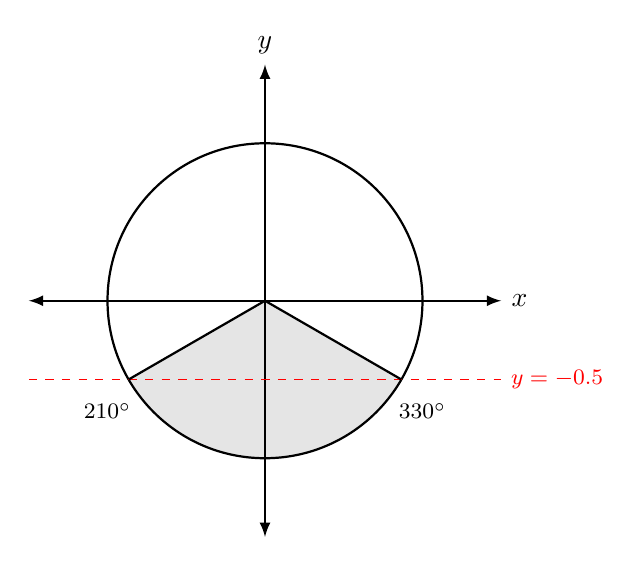
\begin{tikzpicture}[scale=2, >=latex]
            % ==== SHADING ====
            \begin{scope}
                \clip (0,0) -- (210:1) arc (210:330:1) -- cycle;
                \fill[gray!20] (-1.5,-1.5) rectangle (1.5,1.5);
            \end{scope}             
            
            % ==== AXISES ====
            \draw[<->, thick] (-1.5,0) -- (1.5,0) node[right] {$x$};
            \draw[<->, thick] (0,-1.5) -- (0,1.5) node[above] {$y$};

            % ==== UNIT CIRCLE ====
            \draw[thick] (0,0) circle(1);

            % ==== HORIZONTAL LINE y=-0.5 ====
            \draw[dashed, red] (-1.5, -0.5) -- (1.5, -0.5) node[right] {\footnotesize $y=-0.5$};

            % ==== ANGLES ====
            \draw[thick] (0,0) -- (210:1);
            \draw[thick] (0,0) -- (330:1);

            % ==== LABELS ====
            \node at (-1, -0.7) {\footnotesize $210^\circ$};
            \node at (1, -0.7) {\footnotesize $330^\circ$};
        \end{tikzpicture}
    \end{center}

    Z obrázku vidíme, že $\sin x \le -0.5$ platí v intervalu $\left\langle 210^\circ, 330^\circ\right\rangle$.
    \medskip
    Nyní určíme obecné řešení goniometrické nerovnice.
    Kritické body jsou $x_1 = 210^\circ$ a $x_2 = 330^\circ$.
    
    Obecné řešení je tedy:
    \[
    K = \bigcup_{k \in \mathbb{Z}} \left\langle 210^\circ + k \cdot 360^\circ, 330^\circ + k \cdot 360^\circ \right\rangle.
    \]
\end{examplebox}






% -----------------------------------------------------------------
% ---------------------- P Ř Í K L A D Y --------------------------
% -----------------------------------------------------------------

\exercisepart
\setcounter{section}{1}
% =========================
% ÚLOHA 1 – Dokažte pomocí goniometrických vzorců
% =========================
\begin{exercise}[Dokažte I.]
    Dokažte následující goniometrické vztahy pro všechna reálná čísla $x$:
    \begin{tasks}(2)
        \task $\cos \frac{\pi}{12} = \frac{\sqrt{2 + \sqrt{3}}}{2}$
        \task $\sin \frac{\pi}{8} = \frac{\sqrt{2 - \sqrt{2}}}{2}$
        \task $\sin 15^\circ = \frac{\sqrt{2 - \sqrt{3}}}{2}$
        \task $\cos 22^\circ 30' = \frac{\sqrt{2 + \sqrt{2}}}{2}$
    \end{tasks}
\end{exercise}


% =========================
% ÚLOHA 2 – Dokažte pomocí goniometrických vzorců
% =========================
\begin{exercise}[Dokažte II.]
    Dokažte následující goniometrické vztahy pro všechna reálná čísla $x$:
    \begin{tasks}(2)
        \task $\sin x = \frac{2 \tan \frac{\pi}{2}}{1 + \tan^2 \frac{\pi}{2}}$
        \task $\cos x = \frac{1 - \tan^2 \frac{\pi}{2}}{1 + \tan^2 \frac{\pi}{2}}$
        \task $\tan x = \frac{2 \tan \frac{\pi}{2}}{1 - \tan^2 \frac{\pi}{2}}$
        \task $\cot x = \frac{1 - \tan^2 \frac{\pi}{2}}{2 \tan \frac{\pi}{2}}$
    \end{tasks}
\end{exercise}


% =========================
% ÚLOHA 3 – Dokažte pomocí goniometrických vzorců
% =========================
\begin{exercise}[Dokažte III.]
    Dokažte následující goniometrické vztahy pro všechna reálná čísla $x$
    \begin{tasks}(2)
        \task $1 - 2 \sin^2 \frac{x}{2} = \cos x$
        \task $2 \cos^2 \frac{x}{2} - 1 = \cos x$
        \task $1 + \sin x = \left(\sin \frac{x}{2} + \cos \frac{x}{2}\right)^2$
        \task $1 - \cos x = \left(\sin \frac{x}{2} - \cos \frac{x}{2}\right)^2$
    \end{tasks}
\end{exercise}


% =========================
% ÚLOHA 4 – Dokažte pomocí goniometrických vzorců
% =========================
\begin{exercise}[Dokažte IV.]
    Dokažte následující goniometrické vztahy pro všechna reálná čísla $x$:
    \begin{tasks}(2)
        \task $1 + \sin x = 2 \sin^2 \left(\frac{\pi}{4} + \frac{x}{2}\right) = 2 \cos^2 \left(\frac{\pi}{4} - \frac{x}{2}\right)$
        \task $1 - \sin x = 2 \sin^2 \left(\frac{\pi}{4} - \frac{x}{2}\right) = 2 \cos^2 \left(\frac{\pi}{4} + \frac{x}{2}\right)$
        \task $1 + \cos x = 2 \cos^2 \frac{x}{2}$
        \task $1 - \cos x = 2 \sin^2 \frac{x}{2}$
    \end{tasks}
\end{exercise}


% =========================
% ÚLOHA 5 – Upravte goniometrické výrazy pomocí goniometrických vzorců
% =========================
\begin{exercise}[Upravte I.]
    Upravte následující goniometrické výrazy a určete jejich definiční obor:
    \begin{tasks}(2)
        \task $\sin^2 x - \cos^2 x$
        \task $\sin^4 x - \cos^4 x$
        \task $\dfrac{1 - \sin x}{1 + \sin x}$
        \task $\dfrac{1 + \cos x}{1 - \cos x}$
        \task $\left(1 + \sin x\right)\left(1 - \sin x\right)$
        \task $\sin x \cdot \cos^2 x + \sin^3 x$
        \task $\left(\sin x + \cos x\right)^2 - 2\sin x \cos x$
        \task $\left(\cos x - \sin x\right)^2 + \left(\cos x + \sin x\right)^2$
        \task $\dfrac{1}{1 + \cot x} - \dfrac{1}{1 + \tan x}$
        \task $\dfrac{\sin^2 x - \cos^2 x}{\sin x \cos x}$
        \task $\sin^4 x + 2 \sin^2 x \cos^2 x + \cos^4 x$
        \task $\sin^4 x - \cos^4 x + \cos^2 x$
        \task $\dfrac{\sin^2 x - \sin^4 x}{\cos^2 x - \cos^4 x}$
        \task $\dfrac{\cos x}{1 - \sin x} + \dfrac{\cos x}{1 + \sin x}$
        \task $\dfrac{\sin x}{1 + \cos x} + \dfrac{1 + \cos x}{\sin x}$
        \task $\sin^2 x \cdot \cot^2 x + \sin^2 x - 1$
        \task $\cos^2 x \cdot \tan x + \cos^2 x$
        \task $\cos x \cdot \left(\tan x + \cot x\right)$
        \task $\left(1 + \tan^2 x\right)\left(1 - \sin^2 x\right) - \sin^2 x$
        \task $\tan^2 x - \sin^2 x - \tan^2 x \cdot \sin^2 x$
        \task $\cot^2 x - \cos^2 x - \cot^2 x \cdot \cos^2 x$
        \task $1 - \sin^2 x + \cot^2 x \cdot \sin^2 x$        
        \task $\dfrac{\tan x}{1 + \tan^2 x}$
        \task $\dfrac{1}{1 + \tan x} - \dfrac{\cot x}{1 + \cot x}$
        \task $\dfrac{1}{1 + \cot x} - \dfrac{\tan x}{1 + \tan x}$
        \task $\dfrac{\sin^2 x - \cos^2 x}{\sin x \cos x}$

    \end{tasks}
\end{exercise}


% =========================
% ÚLOHA 6 – Upravte a určete D(f)
% =========================
\begin{exercise}[Upravte II.]
    Upravte následující goniometrické rovnosti a určete jejich definiční obor:
    \begin{tasks}(2)
        \task $\cos^4 x - \sin^4 x = \cos^2 x - \sin^2 x$
        \task $\dfrac{\left(\sin x + \cos x\right)^2}{\sin x \cdot \cos x}$
        \task $2 \cos^2 x + 3 \sin x = 0$
        \task $4 \sin^2 x - \tan^2 x = 1$
        \task $2 \cos^2 3x - \sin 3x - 1 = 0$
        \task $\sin^2 x = \sqrt{3} \sin x \cos x$
        \task $\dfrac{1}{\cos^2 x} = 1 + \tan^2 x$
        \task $\dfrac{1}{\sin^2 x} = 1 + \cot^2 x$
        \task $\dfrac{1}{\cos x} - \sin x \cdot \tan x = \cos x$
        \task $\sin x + \cos x = \dfrac{\sin x}{\tan x} + \dfrac{\cos x}{\cot x}$
        \task $\sin x \cot x \cos x = 1 - \sin^2 x$
        \task $\dfrac{\tan^2 x - \sin^2 x}{\sin^2 x} = \tan^2 x$
        \task $\dfrac{2}{\cos^2 x} = \left(1 + \tan^2 x\right)^2 + \left(1 - \tan x\right)^2$
        \task $1 - 2sin^2 x = \dfrac{\cot^2 x - 1}{\cot^2 x + 1}$
        \task $\dfrac{1}{\sin x \cdot \cos x} = \tan x + \cot x$
        \task $\dfrac{1}{\sin^2 x} + \dfrac{1}{\cos^2 x} = \tan^2 x + \cot^2 x$
        \task $\dfrac{1}{\tan^2 x + 1} + \dfrac{1}{\cot^2 x + 1} = 1$
        \task $\tan x - \cot x = \dfrac{1 - 2 \sin^2 x}{\sin x \cos x}$
        \task $\left(\dfrac{1 - \tan x}{1 - \cot x}\right)^2 = \dfrac{1 + \tan^2 x}{1 + \cot^2 x}$
        \task $\left(\dfrac{1 + \tan x}{1 + \cot x}\right)^2 = \dfrac{1 + \tan^2 x}{1 + \cot^2 x}$
        \task \text{$\left(\dfrac{1}{\sin x} + \sin x\right)^2 + \left(\dfrac{1}{\cos x} + \cos x\right)^2 = 5 + \dfrac{1}{\sin^2 x \cdot \cos^2 x}$}
    \end{tasks}
\end{exercise}


% =========================
% ÚLOHA 7 – Upravte a dokažte
% =========================
\begin{exercise}[Upravte a dokažte]
    Upravte následující goniometrické rovnosti a určete jejich definiční obor:
    \begin{tasks}
        \task $\dfrac{1 - \sin x + \cos x}{1 - \sin x} = \dfrac{1 + \sin x + \cos x}{\cos x}$
        \task $\dfrac{1 + \cos x + \sin x}{1 + \cos x} = \dfrac{ 1 + \sin x - \cos x}{\sin x}$
        \task $\dfrac{1 + \sin x - \cos x}{1 - \sin x} = \dfrac{1 - \sin x - \cos x}{\cos x}$
        \task $\dfrac{1 - \cos x + \sin x}{1 + \cos x} = \dfrac{1 - \sin x - \cos x}{\sin x}$
    \end{tasks}
\end{exercise}


\setcounter{section}{2}
% =========================
% ÚLOHA 8 – Řešte rovnice
% =========================
\begin{exercise}[Řešte rovnice]
    Řešte v $\mathbb{R}$ následující rovnice:
    \begin{tasks}(3)
        \task $\sin x = \dfrac{1}{2}$
        \task $\cos x = -\dfrac{\sqrt{2}}{2}$
        \task $\tan x = 1$
        \task $\cot x = -\sqrt{3}$
        \task $\cos x = \dfrac{\sqrt{3}}{2}$
        \task $\sin x = -\dfrac{\sqrt{2}}{2}$
        \task $\sin x = -1$
        \task $\tan x = -1$
        \task $\cos x = \dfrac{1}{2}$
        \task $\cot x = \sqrt{3}$
        \task $2 \sin x - 1 = 0$
        \task $3 \cos x + \sqrt{3} = 0$
        \task $4 \tan x - 4 = 0$
        \task $5 \cot x + 5\sqrt{3} = 0$
        \task $1 - \sin x = 0$
    \end{tasks}
\end{exercise}


% =========================
% ÚLOHA 9 – Řešte rovnice
% =========================
\begin{exercise}[Řešte rovnice II.]
    Řešte v $\mathbb{R}$ následující rovnice:
    \begin{tasks}(2)
        \task $\sin 3x = 1$
        \task $2 \sin^2 x - 1 = 0$
        \task $1 - 2 \cos^2 x = 0$
        \task $3 \tan^2 x - 3 = 0$
        \task $4 - 4 \cot^2 x = 0$
        \task $1 + \sin 2x = 0$
        \task $1 - \cos 2x = 0$
        \task $2 \tan 2x + 2 = 0$
        \task $2 - 2 \cot 2x = 0$
        \task $\sin \left(2x - \dfrac{\pi}{4}\right) = \dfrac{\sqrt{2}}{2}$
        \task $\cos \left(3x + \dfrac{5\pi}{3}\right) = -\dfrac{1}{2}$
        \task $\tan \left(4x - 3\right) = 1$
        \task $\cot \left(5x + 2\right) = -1$
        \task $\cot \left(\dfrac{\pi}{6} - x\right) = \dfrac{\sqrt{3}}{3}$
        \task $\sin \left(1 - x\right) = 0$
        \task $\cos \left(2 + x\right) = -1$
        \task $\sqrt{2} \cos \left(4\pi + 2x\right) = -1$
        \task $3 \sin \left(\dfrac{\pi}{3} - 3x\right) + \dfrac{3}{2} = 0$
        \task $\sin \left(4x - \dfrac{\pi}{3}\right) = \sqrt{2}$
        \task $\tan \left(2x + \dfrac{\pi}{4}\right) = -1$
    \end{tasks}
\end{exercise}


% =========================
% ÚLOHA 10 – Řešte rovnice pomocí substituce
% =========================
\begin{exercise}[Řešte rovnice pomocí substituce]
    Řešte v $\mathbb{R}$ následující rovnice:
    \begin{tasks}(2)
        \task $2 \sin^2 x - 3 \sin x + 1 = 0$
        \task $2 \cos^2 x - \cos x - 1 = 0$
        \task $3 \cos^2 x + 5 \cos x - 2 = 0$
        \task $4 \tan^2 x - 4 \tan x - 8 = 0$
        \task $2 \cot^2 x + 3 \cot x - 5 = 0$
        \task $\sin^2 2x - \sin 2x - 6 = 0$
        \task $4 \sin^2 x - 2 \sin x = \sqrt{3}\left(-1 + 2 \sin x\right)$
        \task $2 \sin^2 x + 3 \cos x = 0$
        \task $2 \sin^2 x + 3\sqrt{2} \cos x - 7 = 0$
        \task $\sin^2 x - \cos^2 x + \sqrt{3} - 2 = 0$
        \task $12 \sin^4 x + \sin^2 x - 1 = 0$
        \task $2 \cos^4 x - 3 \cos^2 x + 1 = 0$
        \task $8 \cos^4 x - 10 \cos^2 x + 3 = 0$
        \task $\tan^2 x - \tan x - 2 = 0$
        \task $\tan x + \cot x - 2 = 0$
        \task $\tan^2 x + 3 \cot x - 4 = 0$
        \task $3 \cot^2 x - \cot x - 4 = 0$
        \task $2 \sin^2 3x - 5 \sin 3x + 2 = 0$
        \task $4 \cos^2 2x + \cos 2x - 3 = 0$
        \task $3 \tan^2 4x - \tan 4x - 4 = 0$
        \task $2 \cot^2 5x + \cot 5x - 3 = 0$
        \task $2 \sin^2 x + \sin x \cos x - 1 = 0$
        \task $12 \sin^4 x + sin^2 - 1 = 0$
        \task $8 \cos^4 x - 10 \cos^2 x + 3 = 0$
        \task $3 \tan^2 x - \tan x - 4 = 0$
        \task $4 \cot^2 x + \cot x - 3 = 0$
        \end{tasks}
\end{exercise}


% ========================
% ÚLOHA 11 – Řešte rovnice pomocí substituce
% =========================
\begin{exercise}[Řešte rovnice pomocí substituce II.]
    Řešte v $\mathbb{R}$ následující rovnice:
    \begin{tasks}(2)
        \task $\left(\sin 2x + \cos 2x\right)^2 = 0,5$
        \task $\left(\sin 2x - \cos 2x\right)^2 = 1 - \dfrac{\sqrt{3}}{2}$
        \task $\sin 2x \cdot \cos 2x = \dfrac{1}{2}$
        \task $\sin 2x \cdot \cos 2x = -\dfrac{\sqrt{3}}{4}$
        \task $\sin^2 2x + \cos^2 2x = 1$
        \task $\sin^2 2x - \cos^2 2x = \dfrac{1}{2}$
        \task $\dfrac{1 + \sin 2x}{\cos 2x} = \left(\cos x + \sin x\right)^2$
        \task $\dfrac{1 - \sin 2x}{\cos 2x} = \left(\cos x - \sin x\right)^2$
        \task $\tan x + \cot x = 2 \cdot \sin 2x$
        \task $\tan x + \cot x = 8 \cdot \cos 2x$
        \task $\tan x \cdot \cos^2 x \cdot \cos 2x = -\dfrac{1}{8}$
        \task $\cot x \cdot \sin^2 x \cdot \cos 2x = \dfrac{1}{4}$
        \task $\tan x \cdot \left(1 - \sin 2x\right) = 1 - \cos 2x$
        \task $\cot x \cdot \left(1 + \sin 2x\right) = 1 + \cos 2x$
        \task $\dfrac{1}{\cos^2 2x} - 2\tan 2x = 0$
        \task $\dfrac{1}{\sin^2 2x} + 2\cot 2x = 0$
    \end{tasks}
\end{exercise}


% =========================
% ÚLOHA 12 – Řešte rovnice
% =========================
\begin{exercise}[Řešte rovnice III.]
    Řešte v $\mathbb{R}$ následující rovnice:
    \begin{tasks}(2)
        \task $\sin 2x + \cos 3x = 0$
        \task $2 \sin 2x - \cos 3x = 0$
        \task $2 \sin 2x + 3 \cos 3x = 0$
        \task $3 \sin 3x - 2 \cos 2x = 0$
        \task $\sin 4x + \sqrt{2} \sin 2x = 0$
        \task $\cos 4x - \sqrt{2} \cos 2x = 0$
        \task $\sin 4x + \sin 2x = 0$
        \task $\sin 4x + 2 \sin^2 2x = 2$
        \task $\cos 4x - \cos 2x = 0$
        \task $1 + \cos 4x = \cos 2x$
        \task $\left(1 + \cos 4x\right) \cdot \sin 2x = \cos 2x$
        \task $\cos 4x - 3 \cos 2x - 3 \sin 2x = 0$
        \task $\text{$2 \sin^4 2x - \sin^2 2x \cdot \sin 4x = 2 \sin^2 2x - \sin 4x$}$
    \end{tasks}
\end{exercise}


% =========================
% ÚLOHA 13 – Řešte rovnice
% ========================
\begin{exercise}[Řešte rovnice IV.]
    Řešte v $\mathbb{R}$ následující rovnice:
    \begin{tasks}(2)
        \task $\sin \left(x + 30^\circ\right) + \sin \left(x - 30^\circ\right) = \dfrac{\sqrt{3}}{2}$
        \task $\sin x + \sin\left(x + \dfrac{\pi}{3}\right) = - \dfrac{\sqrt{3}}{2}$
        \task $\cos \left(x + 45^\circ\right) + \cos \left(x - 45^\circ\right) = 1$
        \task $\sin \left(\dfrac{\pi}{x} + x\right) - \sin \left(\dfrac{\pi}{4} - x\right) = \sin 2x$
        \task $\sin \left(x - \dfrac{\pi}{6}\right) = \sin x - \sin \dfrac{\pi}{6}$
        \task $\cos \left(x + \dfrac{\pi}{3}\right) - \cos \left(x - \dfrac{\pi}{3}\right) = 1$
        \task $\tan \left(x + 45^\circ\right) + \tan \left(x - 45^\circ\right) = 2$
        \task \text{$\sin \left(x + 30^\circ\right) + \cos\left(x + 60^\circ\right) = 1 + \cos 2x$}
        \task \text{$\sin \left(x - 60^\circ\right) - \cos\left(x - 30^\circ\right) = \sin 2x - 1$}
        \task $\sin x - 2 \sin \left(60^\circ - x\right) = 0$
        \task $\cos x + \sqrt{3} \cos \left(30^\circ + x\right) = 0$
        \task $\tan \left(x + 30^\circ\right) + \tan \left(30^\circ - x\right) = 2$
        \task $\sin \left(x + \dfrac{\pi}{4}\right) = 5 \cos \left(s - \dfrac{\pi}{4}\right)$
        \task $\tan \left(x + \dfrac{\pi}{6}\right) \cdot \tan \left(x - \dfrac{\pi}{4}\right) = \dfrac{1}{4}$
        \task $\cos \left(x + \dfrac{\pi}{3}\right) + \cos \left(x - \dfrac{\pi}{6}\right) = 1$
        \task $\cos \left(x + 60^\circ\right) \cdot \cos \left(x - 60^\circ\right) = \dfrac{1}{4}$
        \task $\sin \left(x + 45^\circ\right) - \sin \left(45^\circ - x\right) = \sqrt{2} \cos 2x$
        \task $\sin \left(x + \dfrac{\pi}{4}\right) \cdot \cos \left(x + \dfrac{\pi}{4}\right) = \dfrac{1}{4}$
    \end{tasks}
\end{exercise}


% =========================
% ÚLOHA 14 – Řešte rovnice
% =========================
\begin{exercise}[Řešte rovnice V.]
    Řešte v $\mathbb{R}$ následující rovnice:
    \begin{tasks}(2)
        \task $\sin^{3} x - \cos^{3} x = \sin^{2} x - \cos^{2} x$
        \task $\sin^{3} x + \cos^{3} x = \sin^{2} x - \cos^{2} x$
        \task $\sin x + \cos x = \cos 2x$
        \task $\sin x - \cos x = \sin 2x$

        \task $\sin^{2} x + \sin 2x = \cos^{2} x$
        \task $\sin^{3} x + 0{,}5 \sin 2x = 1 - \cos^{3} x$
        \task $\cot x + \dfrac{\sin x}{1 + \cos x} = 1$
        \task $\sin^{4} x + \cos^{4} x = 0{,}5$

        \task $\sin^{6} x + \cos^{6} x = 0{,}25$
        \task $\cot x - 1 = \dfrac{4 \cos 2x}{1 + \tg x}$
        \task $\sin x + \cos x = \dfrac{1}{2}$
        \task $\sin x - \cos x = \dfrac{1}{2}$

        \task $\dfrac{1}{\sin x} = \sin x + \cos x$
        \task $\dfrac{2}{\sin x} = \sin x + \cos x$
        \task $2 \sin x = \dfrac{3(1 + \cos x)}{\sin x}$
        \task $(1 - \tg x)(1 + \sin 2x) = 1 + \tg x$

        \task $\cos x + \cot x = 1 + \sin x$
        \task $\cos 2x = \cos^{2} x - 0{,}5 \tg^{2} x$
        \task $\tg x \left( \tg x + \dfrac{1}{\cos x} \right) = 1$
        \task $\dfrac{3}{\sin^{2} x} - 2 = 4 \cot x$

        \task $\dfrac{1 + \cot x}{1 - \cot x} = 2 \sin 2x$
        \task $\dfrac{1 - \cot x}{1 + \cot x} = 2 \cos 2x$
        \task $\dfrac{1 + \tg x}{1 - \tg x} = 2 \cos 2x$
        \task $\dfrac{1}{\sin^{2} x} + 2 \cot x = 0$

        \task $\dfrac{1}{\cos^{2} x} + \sqrt{3} \tg x = 1$
        \task $\tg \left(\frac{\pi}{2} + x\right) - \cot^{2} x
              = \dfrac{\cos 2x - 1}{\sin^{2} x}$
    \end{tasks}
\end{exercise}


% =========================
% ÚLOHA 15 – Řešte nerovnice
% =========================
\begin{exercise}[Řešte nerovnice]
    Řešte v $\mathbb{R}$ následující nerovnice:
    \begin{tasks}(2)
        \task $\sin x > 0$
        \task $\cos x \le 0$
        \task $\tan x < 1$
        \task $\cot x \ge -1$
        \task $1 + \sin x > 0$
        \task $1 - \cos x < 1$
        \task $2 \sin^2 x - 1 > 0$
        \task $1 - 2 \cos^2 x \le 0$
        \task $\sin 2x + \cos 2x > 0$
        \task $\sin 2x - \cos 2x < 1$
        \task $\tan x + \cot x \ge 2$
        \task $\tan x - \cot x < 0$
    \end{tasks}
\end{exercise}


% =========================
% ÚLOHA 16 – Řešte nerovnice
% =========================
\begin{exercise}[Řešte nerovnice II.]
    Řešte v $\mathbb{R}$ následující nerovnice:
    \begin{tasks}(2)
        \task $2 \sin x + \sqrt{3} < 0$
        \task $3 \cos x - 1 \ge 0$
        \task $4 \tan x + 4 > 0$
        \task $5 \cot x - 5\sqrt{3} \le 0$
        \task $\sin 2x - 1 < 0$
        \task $\cos 2x + 1 \ge 0$
        \task $2 \tan 2x - 2 < 0$
        \task $2 \cot 2x + 2 \ge 0$
        \task $\sin^2 x - \cos^2 x > 0$
        \task $\sin^2 x + \cos^2 x < 1$
        \task $\tan^2 x - 1 \ge 0$
        \task $\cot^2 x + 1 > 2$
    \end{tasks}
\end{exercise}


% =========================
% ÚLOHA 17 – Řešte nerovnice
% =========================
\begin{exercise}[Řešte nerovnice III.]
    Řešte v $\mathbb{R}$ následující nerovnice:
    \begin{tasks}(2)
        \task $2 \sin^2 x > 3 \cos x$
        \task $\sin^2 x + 3 \cos x - 3 \le 0$
        \task $\tan^2 x + \cot^2 x > 2$
        \task $\sin^2 x + 2 \sin x \cos x + \cos^2 x > \frac{1}{2}$
        \task $\sin \left(2x - \dfrac{\pi}{4}\right) > \dfrac{\sqrt{2}}{2}$
        \task $\cos \left(3x + \dfrac{5\pi}{3}\right) < -\dfrac{1}{2}$
        \task $\tan \left(4x - 3\right) \ge 1$
        \task $\cot \left(5x + 2\right) \le -1$
    \end{tasks}
\end{exercise}

% =========================
% Test VS Code Remote SSH + Git
% =========================


% =========================
% ÚLOHA X - BONUS: rovnice
% =========================
\begin{exercise}[BONUS: řešte rovnice]
    Řešte v $\mathbb{R}$ následující rovnice:
    \begin{tasks}(2)
        \task $9^{\sin^2 x} \cdot 3^{\cos^2 x} = 1$
        \task $5^{\tan x} \cdot 5^{\cot x} = 25$

    \end{tasks}
    
\end{exercise}


% =========================
% ÚLOHA Y - BONUS: důkaz součtových vzorců
% =========================
\begin{exercise}[BONUS: Dokažte součtové vzorce]
    Dokažte následující goniometrické vztahy pro všechna reálná čísla $x$ a $y$:
    \begin{tasks}
        \task $\sin (x - y) = \sin x \cos y - \cos x \sin y$
        \task $\cos (x + y) = \cos x \cos y - \sin x \sin y$
    \end{tasks}
\end{exercise}


\end{document}